\documentclass[journal,10pt,twocolumn]{article}
\usepackage{graphicx}
\usepackage[margin=0.5in]{geometry}
\usepackage{amsmath}
\usepackage{array}
\usepackage{booktabs}
\usepackage{enumerate}
\providecommand{\norm}[1]{\left\lVert#1\right\rVert}
\providecommand{\abs}[1]{\left\vert#1\right\vert}
\let\vec\mathbf
\newcommand{\myvec}[1]{\ensuremath{\begin{pmatrix}#1\end{pmatrix}}}
\newcommand{\mydet}[1]{\ensuremath{\begin{vmatrix}#1\end{vmatrix}}}
\providecommand{\brak}[1]{\ensuremath{\left(#1\right)}}
\title{\textbf{Matrix Assignment}}
\author{Mannava Venkatasai}
\date{September 2022}

\begin{document}

\maketitle
\paragraph{\textit{Problem Statement} - The length of a tangent from a point A at distance 5 cm from the centre of the circle is 4
cm. Find the radius of the circle.}
\begin{enumerate}
	\item \textbf{PO = 5cm}
	\item \textbf{PQ = 4cm}
\end{enumerate}
\begin{figure}[h]
\centering
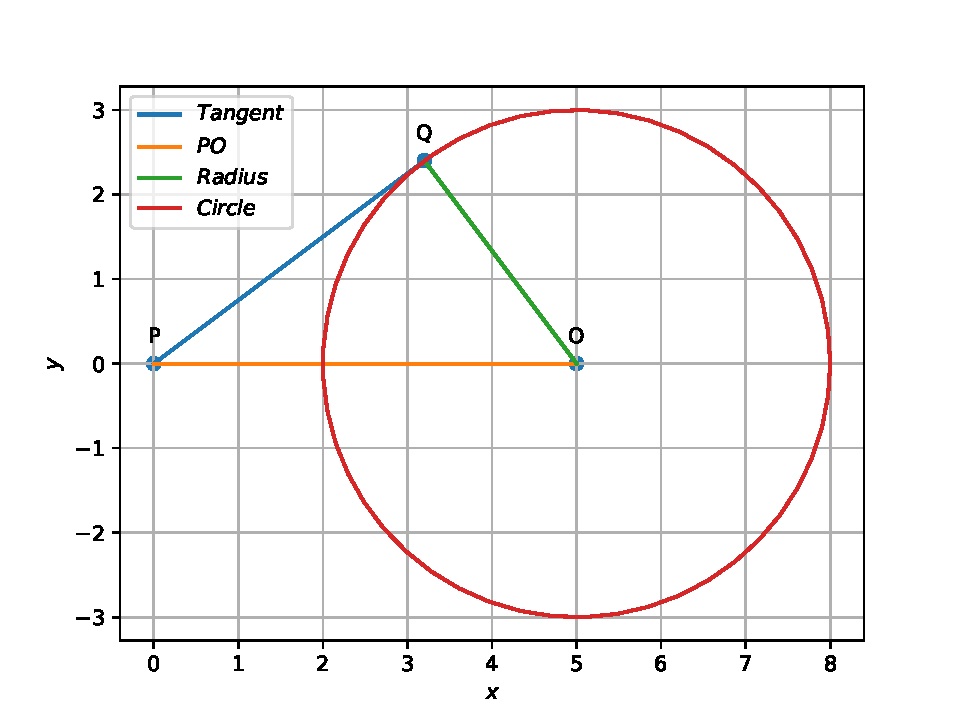
\includegraphics[width=1\columnwidth]{circle.pdf}
\caption{Circle with centre O and a tangent is drawn to circle from point P to Q}
\label{fig:Circle}
\end{figure}

\section*{Solution}
\subsection*{Part 1}
\section*{Construction}
The input parameters are the lengths of AB and AD and angle between AB and ADs \vspace{2mm}\\
{
\setlength\extrarowheight{2pt}
\begin{tabular}{|c|c|c|}
 \hline
 \textbf{Symbol}&\textbf{Value}&\textbf{Description}\\
 \hline
 a&4&PQ\\
 \hline
 d&5&OP\\
 \hline
	$\theta$&$\arccos(4/5)$&$\angle$P\\
 \hline
 0&$d%
 \begin{pmatrix}
  cos(0)\\
  sin(0)\\
 \end{pmatrix}$%
 &centre\\
 \hline
 Q&$a%
 \begin{pmatrix}
  cos\theta\\
  sin\theta\\
 \end{pmatrix}$%
 &point of contact\\
 \hline
\end{tabular}
}
\subsection*{Part 2}
We know that the angle made by tangent and radius of circle at the point of contact is 90 degrees. \\
In order to get the radius of circle consider the triangle $\triangle$PQO \\
\begin{align}
	r = \norm{\vec{O}-\vec{Q}}
\end{align}
\begin{align}
	\norm{\vec{O} - \vec{Q}}= 3
\end{align}
\begin{align}
  r= 3 cm 
\end{align}


Hence the radius of circle is 3cm

\subsection*{Part 3}
Let us proove that the angle made by the tangent and radius at the point of contact is 90  degrees. \\
\begin{enumerate}
	\item OC=OA=3cm
	\item AB = 4cm
\end{enumerate}
\begin{figure}[h]
\centering
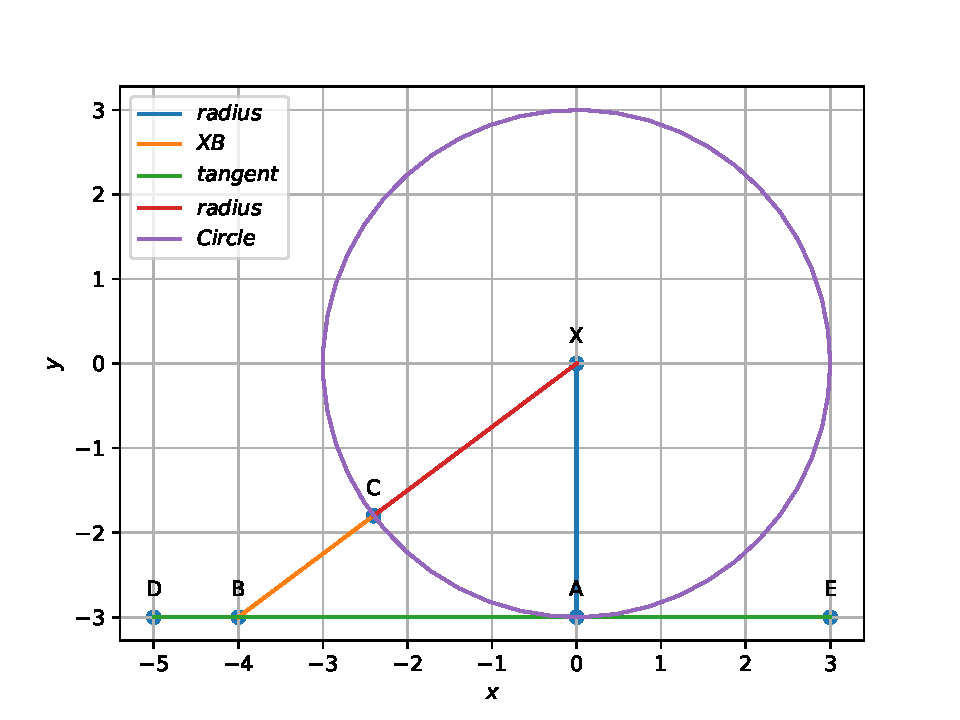
\includegraphics[width=1\columnwidth]{proof.pdf}
\caption{Circle with centre X and a tangent is drawn to circle from point B to A}
\label{fig:Circle}
\end{figure}
From the above figure 
\begin{align}
	\norm{\vec{XB}} = \norm{\vec{XC}} + \norm{\vec{CB}}
\end{align}
\begin{align}
	\norm{\vec{B-X}} = \norm{(\vec{C-X})} + \norm{(\vec{B-C})}
\end{align}
we know that \\
\begin{align}
	\norm{\vec{A-X}} = \norm{\vec{C-X}}
\end{align}
From the above equation we can say that 
\begin{align}
	\norm{\vec{B-X}} > \norm{\vec{A-X}}
\end{align}
From the above result we can conclude that the distance between centre of circle to the any point on the tangent other than point of contact is greater than the distance between the centre to the point of contact. \\
XA is the shortest distance
Hence The distance from centre to the point of contact is shortest distance.\\
Shortest distance of a point from a given line is the perpendicular distance from that line.\\
Hence prooved.
\end{document}
